\documentclass[conference]{IEEEtran}

% Make ligatures and symbols extract correctly as text (pdfLaTeX only)
\ifdefined\pdfgentounicode
  \input{glyphtounicode}
  \pdfgentounicode=1
\fi

\usepackage{cite}
\usepackage{amsmath,amssymb}
\usepackage{graphicx}
\usepackage{booktabs}
\usepackage{xcolor}
\usepackage{tikz}
\usetikzlibrary{positioning,arrows.meta}
\usepackage{pgfplots}
\pgfplotsset{compat=1.18}
\usepackage{url}
\usepackage[hidelinks]{hyperref}
\hypersetup{
  pdftitle={Orbital Sentinel: An Open, Cross-Checked Pipeline for Satellite Conjunction Assessment with Cascade-Aware Maneuver Planning},
  pdfauthor={Soumyadeep Dey, Pritam Patra, Subarna Maity, Sourish Panda},
  pdfsubject={Space situational awareness; conjunction assessment},
  pdfkeywords={collision avoidance, collision probability, conjunction assessment, explainable machine learning, orbital debris, space situational awareness, SGP4, XGBoost}
}

\newcommand{\Pc}{P_c}
\newcommand{\bvec}[1]{\mathbf{#1}}
\newcommand{\norm}[1]{\left\|#1\right\|}
\newcommand{\HBR}{R_{\mathrm{HB}}}
\newcommand{\rr}{\bvec{r}_{\mathrm{r}}}
\newcommand{\vr}{\bvec{v}_{\mathrm{r}}}

\pgfplotsset{every axis/.append style={font=\footnotesize}}

\begin{document}

\title{Orbital Sentinel: An Open, Cross-Checked Pipeline for Satellite
Conjunction Assessment with Cascade-Aware Maneuver Planning}

\author{
\IEEEauthorblockN{Soumyadeep Dey\IEEEauthorrefmark{1},
Pritam Patra\IEEEauthorrefmark{2},
Subarna Maity\IEEEauthorrefmark{3}, and
Sourish Panda\IEEEauthorrefmark{3}}
\IEEEauthorblockA{\IEEEauthorrefmark{1}\textit{Dept. of Computer Applications},
\IEEEauthorrefmark{2}\textit{Dept. of Computer Science and Engineering},
\IEEEauthorrefmark{3}\textit{Dept. of Information Technology}\\
\textit{Guru Nanak Institute of Technology}, Howrah, West Bengal, India\\
ORCID: 0009-0007-9118-8844 (S. Dey), 0009-0009-6054-3748 (S. Maity),
0009-0001-4549-5268 (S. Panda)}
}

\maketitle

\begin{abstract}
As the tracked catalog grows, satellite operators must screen more object
pairs and justify each maneuver decision. This paper presents Orbital Sentinel,
an open-source pipeline that screens a two-line element (TLE) catalog for close
approaches over a 24-h horizon, computes the Foster two-dimensional probability
of collision using per-object hard-body radii and a covariance that grows with
TLE age, and streams the results to a three-dimensional web globe. Every
probability is cross-checked against the Chan series and the Alfano
maximum-probability bound, and the highest-risk alerts are also checked by Monte
Carlo sampling. Candidate avoidance burns are verified by re-propagation, and the
best candidates are re-screened against the whole catalog and simulated debris,
so a burn that creates a secondary conjunction is rejected. Collision
consequences are modeled with the NASA Standard Breakup Model and fragment
propagation under J2 and drag. An XGBoost surrogate of the logarithmic
probability, explained with TreeSHAP, never changes the published probability
and can only escalate, never lower, the physics-based action. On 12\,000
held-out synthetic encounters it attains a mean absolute error of 0.106 decades,
with 0.975 precision and 0.950 recall at the $10^{-4}$ maneuver threshold,
whereas a miss-distance-only baseline detects no high-risk encounter. Screening
500 objects takes about 1~s on a laptop processor, and all 18 analytical physics
checks and 204 regression tests pass.
\end{abstract}

\begin{IEEEkeywords}
collision avoidance, collision probability, conjunction assessment, explainable
machine learning, orbital debris, space situational awareness, SGP4, XGBoost
\end{IEEEkeywords}

%% ==========================================================================
\section{Introduction}
\label{sec:intro}

According to the European Space Agency (ESA), about 1.5 million objects
between 1 and 10~cm are in orbit, and about 47\,000 objects are regularly
tracked and cataloged~\cite{esa2026,esastats2026}. The 2009 collision between
Iridium~33 and Cosmos~2251 created thousands of trackable
fragments~\cite{kelso2009}, and collisions are expected to dominate future
debris growth through the cascade described by Kessler and
Cour-Palais~\cite{kessler1978,liou2006}.

Operational conjunction assessment (CA) relies on precise orbit data, the
two-dimensional probability of collision ($\Pc$), and expert
review~\cite{nasa2020}. Open tools for education, prototyping, and research
rarely expose the complete chain from screening to probability to maneuver
decision. Two gaps are common. First, operational practice screens a planned
maneuver against the full catalog before execution~\cite{nasa2020}, but open
research tools rarely implement this step and often check a burn only against
the primary threat, so a burn that resolves one conjunction can create another.
Second, machine-learning (ML) components are increasingly proposed for
CA~\cite{uriot2022,sanchez2021,stevenson2023}, but their outputs are rarely
explained or prevented from lowering physically derived risk.

This paper presents Orbital Sentinel, an open-source system that addresses both
gaps. Its contributions are:
\begin{enumerate}
  \item a 24-h future-window screening pipeline that combines a spatial-index
        candidate search, a linear relative-motion filter, and Brent refinement
        of the time of closest approach (TCA);
  \item a Foster $\Pc$ engine with a TLE-age covariance model and per-object
        hard-body radius (HBR), cross-checked on every alert by the Chan series
        and the Alfano bound and, for the highest-risk alerts, by Monte Carlo
        sampling;
  \item a cascade-aware maneuver planner that re-propagates every candidate
        burn and re-screens the best candidates against the full catalog and
        simulated fragments;
  \item an explainable XGBoost $\Pc$ surrogate whose held-out accuracy,
        baselines, and per-alert TreeSHAP attributions are reported, and which
        can raise but never lower the physics-based action; and
  \item a reproducible evaluation, including negative results that justify
        keeping weaker learned components out of the decision path.
\end{enumerate}
Our evaluation is internal: it checks consistency against analytical
solutions, independent numerical references, and synthetic data, not
operational skill.

%% ==========================================================================
\section{Related Work}
\label{sec:related}

\textit{Orbit propagation and screening.} Public TLEs are propagated with the
Simplified General Perturbations~4 (SGP4) model~\cite{hoots1980}, whose
reference implementation was revised by Vallado \textit{et
al.}~\cite{vallado2006}. SGP4 accuracy degrades with element
age~\cite{flohrer2008,vallado2012}. Classical screening first removes pairs
whose apogee/perigee shells cannot overlap~\cite{hoots1984}.

\textit{Collision probability.} For short encounters with linear relative
motion, $\Pc$ reduces to a two-dimensional Gaussian integral over the hard-body
disk in the encounter plane, introduced by Foster and
Estes~\cite{foster1992}. Equivalent formulations include the Chan
series~\cite{chan2008} and the contour integral of Patera~\cite{patera2001}.
Akella and Alfriend~\cite{akella2000} formalized the short-encounter
assumptions, and Alfriend \textit{et al.}~\cite{alfriend1999} showed how
strongly $\Pc$ depends on covariance error. NASA's Conjunction Assessment Risk Analysis (CARA)
program has documented the usage boundaries of the two-dimensional
method~\cite{hall2019}, Monte Carlo verification~\cite{hall2018}, and
operational practice, including the $10^{-4}$ maneuver
threshold~\cite{nasa2020}. Open implementations cover parts of this chain:
CARA publishes its probability tools as open source~\cite{caratools}, and the
SOCRATES service publishes TLE-based conjunction screening
reports~\cite{kelso2006}. To our knowledge, none couples screening,
probability, breakup, and catalog-wide maneuver re-screening in one open
pipeline.

\textit{Machine learning for CA.} The ESA Collision Avoidance Challenge
trained models to forecast the final risk in a sequence of conjunction data
messages (CDMs)~\cite{uriot2022}. Other work combined ML with evidence
theory~\cite{sanchez2021}, benchmarked deep networks for all-vs-all
screening~\cite{stevenson2023}, and corrected orbit-prediction
error~\cite{peng2020}. These studies rarely report feature attributions or
limit a model's authority over the physical estimate. We use the exact tree
form of Shapley additive explanations, TreeSHAP~\cite{lundberg2020}, with
gradient-boosted trees~\cite{chen2016}, and keep the physical $\Pc$
authoritative.

\textit{Debris and cascades.} The NASA Standard Breakup Model
(SBM)~\cite{johnson2001} is the standard tool for generating fragment
populations. Graph neural networks~\cite{velickovic2018} suggest learned
formulations of cascade risk; we use a physics-first graph and evaluate learned
graph rankers only as advisory cross-checks.

%% ==========================================================================
\section{System Architecture}
\label{sec:arch}

Fig.~\ref{fig:pipeline} shows the pipeline. A Python backend (FastAPI)
propagates the catalog, refreshes alerts every 30~s and after every state
change, and serves a representational state transfer (REST) application
programming interface (API) together with a WebSocket stream that pushes
positions at 1~Hz. A React client renders objects, encounter hotspots, and
debris on a CesiumJS globe, converting inertial coordinates to Earth-fixed ones
with Greenwich mean sidereal time~\cite{vallado2006}. TLEs come from
Space-Track when credentials are configured, then from a public mirror, and
otherwise from a bundled 31\,068-object snapshot. All physics runs on a
simulation clock, defined as wall-clock time plus an operator offset of up to
$\pm24$~h, so scenarios are repeatable. Every assumed input, such as an
object's mass or radius, is a named constant, and each output records which
assumption it used.

\begin{figure}[!t]
\centering
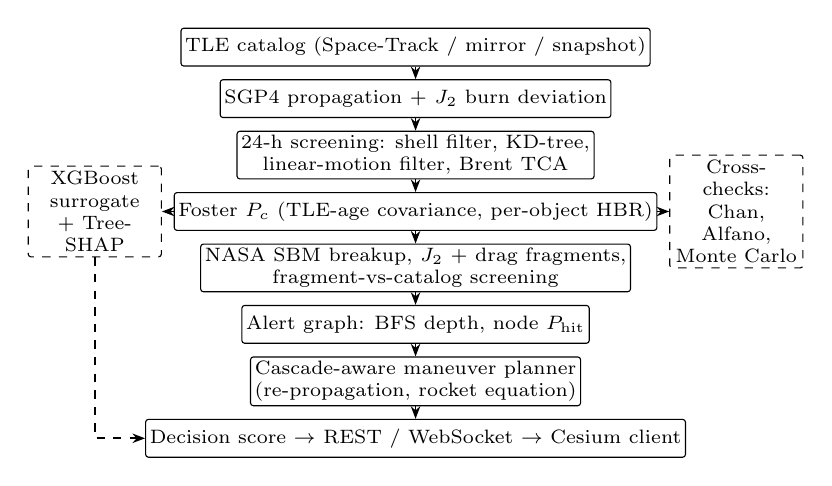
\begin{tikzpicture}[
  font=\scriptsize,
  box/.style={draw, rounded corners=1pt, align=center, minimum width=3.9cm,
              minimum height=0.48cm, inner sep=1.5pt},
  side/.style={draw, dashed, rounded corners=1pt, align=center,
               text width=1.55cm, inner sep=2pt},
  arr/.style={-{Stealth[length=1.6mm]}, semithick},
  node distance=0.16cm]
\node[box] (tle) {TLE catalog (Space-Track / mirror / snapshot)};
\node[box, below=of tle] (prop) {SGP4 propagation + $J_2$ burn deviation};
\node[box, below=of prop] (scr) {24-h screening: shell filter, KD-tree,\\
      linear-motion filter, Brent TCA};
\node[box, below=of scr] (pc) {Foster $P_c$ (TLE-age covariance, per-object HBR)};
\node[box, below=of pc] (sbm) {NASA SBM breakup, $J_2$ + drag fragments,\\
      fragment-vs-catalog screening};
\node[box, below=of sbm] (casc) {Alert graph: BFS depth, node $P_{\mathrm{hit}}$};
\node[box, below=of casc] (man) {Cascade-aware maneuver planner\\
      (re-propagation, rocket equation)};
\node[box, below=of man] (dec) {Decision score $\rightarrow$ REST / WebSocket
      $\rightarrow$ Cesium client};
\node[side, left=0.15cm of pc] (ml) {XGBoost surrogate\\+ TreeSHAP};
\node[side, right=0.15cm of pc] (chk) {Cross-checks:\\Chan, Alfano,\\Monte Carlo};
\foreach \a/\b in {tle/prop, prop/scr, scr/pc, pc/sbm, sbm/casc, casc/man, man/dec}
  \draw[arr] (\a) -- (\b);
\draw[arr] (pc) -- (ml);
\draw[arr] (pc) -- (chk);
\draw[arr, dashed] (ml) |- (dec);
\end{tikzpicture}
\caption{Orbital Sentinel pipeline. Solid boxes produce authoritative
quantities. Dashed boxes are verification or learned outputs that never modify
the physical $P_c$; the surrogate feeds the decision score and can only
escalate the action.}
\label{fig:pipeline}
\end{figure}

%% ==========================================================================
\section{Methods}
\label{sec:method}

\subsection{Propagation and Executed Burns}

States are propagated with SGP4, using World Geodetic System 1972 (WGS-72)
constants in the true-equator mean-equinox frame~\cite{hoots1980,vallado2006}.
Refitting a TLE after a maneuver would introduce fitting error, so an executed
impulse $\Delta\bvec{v}$ is applied as a deviation computed with a two-body plus
Earth-oblateness ($J_2$) integrator (fourth-order Runge--Kutta):
\begin{equation}
  \bvec{r}(t) = \bvec{r}_{\mathrm{SGP4}}(t)
  + \left[\bvec{r}_{J_2}\big(t;\bvec{x}_0+[\bvec{0};\Delta\bvec{v}]\big)
          - \bvec{r}_{J_2}(t;\bvec{x}_0)\right],
\label{eq:burn}
\end{equation}
where $\bvec{x}_0$ is the position--velocity state at burn time. A zero burn
therefore leaves the trajectory unchanged, and the planner and the executed burn
share one model.

\subsection{Future-Window Screening}

All objects are propagated on a 60-s grid over 24~h. An apogee/perigee shell
filter removes objects whose radial range cannot overlap any other
object~\cite{hoots1984}. At each step $t_k$, candidate pairs are found with a
$k$-dimensional tree (KD-tree)~\cite{bentley1975} using the search radius
\begin{equation}
  \rho = d_{\mathrm{th}} + \tfrac{1}{2}\,v_{\mathrm{max}}\,\Delta t,
\end{equation}
with threshold $d_{\mathrm{th}}=25$~km, step $\Delta t=60$~s, and
$v_{\mathrm{max}}$ equal to twice the largest orbital speed in the window. Each
candidate is passed through a linear relative-motion filter. With relative
position $\rr$ and relative velocity $\vr$, the local closest-approach time is
\begin{equation}
  t^{*} = -\frac{\rr\cdot\vr}{\norm{\vr}^{2}},
\end{equation}
and the candidate is kept if $|t^{*}|\le\Delta t/2$ and
$\norm{\rr+\vr\,t^{*}}\le d_{\mathrm{th}}+5$~km. Slow co-orbital pairs
($\norm{\vr}<0.05$~km/s) skip the $t^{*}$ test, and at most three candidate
steps per pair are refined, smallest linearized miss first. The TCA is refined
by bounded Brent minimization~\cite{brent1973,virtanen2020} of the exact SGP4
distance on $[t_k-\Delta t,\,t_k+\Delta t]$ with 1-ms tolerance, and the
closest encounter per pair within $d_{\mathrm{th}}$ becomes an alert.

\subsection{Covariance Model and Foster Probability}

TLEs carry no covariance, so a per-object covariance is modeled in the
radial, transverse, and normal (RTN) frame. Its 1$\sigma$ values grow linearly
with the propagation span $\tau$ (days) from the TLE epoch to the TCA:
\begin{equation}
\begin{aligned}
  \boldsymbol{\sigma}(\tau) &= \boldsymbol{\sigma}_0 + \bvec{g}\,\tau,\qquad
  \boldsymbol{\sigma}_0=(0.10,\,0.50,\,0.15)~\text{km},\\
  \bvec{g} &= (0.10,\,1.00,\,0.10)~\text{km/day}.
\end{aligned}
\label{eq:cov}
\end{equation}
This is a single, regime-independent simplification chosen to match the order
of magnitude of low-Earth-orbit TLE errors~\cite{flohrer2008,vallado2012};
actual errors vary with orbit regime and drag, so absolute $\Pc$ values are
indicative. Each covariance is rotated to the inertial frame,
$\bvec{C}=\bvec{R}\,\mathrm{diag}(\boldsymbol{\sigma}^2)\bvec{R}^{T}$, and the
two are summed. The encounter plane is normal to $\vr$. With unit vectors
$\hat{\bvec{h}}=\vr/\norm{\vr}$,
$\hat{\bvec{t}}\propto\hat{\bvec{h}}\times\bvec{r}_1$, and
$\hat{\bvec{n}}=\hat{\bvec{t}}\times\hat{\bvec{h}}$, the projection
$\bvec{B}=[\hat{\bvec{t}}\;\hat{\bvec{n}}]^{T}$ gives the miss vector
$\bvec{b}=\bvec{B}\rr$ and the encounter covariance
$\bvec{C}_B=\bvec{B}(\bvec{C}_1+\bvec{C}_2)\bvec{B}^{T}$. Foster's
probability~\cite{foster1992} is
\begin{equation}
  \Pc=\frac{1}{2\pi\sqrt{|\bvec{C}_B|}}\iint_{\norm{\bvec{x}}\le\HBR}
  e^{-\frac{1}{2}(\bvec{x}-\bvec{b})^{T}\bvec{C}_B^{-1}(\bvec{x}-\bvec{b})}
  \,d\bvec{x}.
\label{eq:foster}
\end{equation}
It is evaluated in polar coordinates with 48-point Gauss--Legendre quadrature
in radius and a 96-point trapezoid rule in angle. The combined radius $\HBR$ is
the sum of the objects' radii. Each radius is taken from the radar
cross-section class in the public satellite catalog (SATCAT): 0.18~m for small
and 0.56~m for medium objects. Otherwise it defaults by object type: 5~m for
payloads, 4~m for rocket bodies, 0.5~m for debris, and 1~m for unknown objects.
Named large structures have their own values, for example 55~m for the
International Space Station. An alert is flagged when the short-encounter
assumption is questionable
($\norm{\vr}<0.1$~km/s)~\cite{akella2000,hall2019}.

\subsection{Independent Probability Cross-Checks}

Each alert also carries independent estimates computed from its published
encounter-plane fields (miss vector, $3\sigma$ ellipse, and HBR). The first is
the Chan equivalent-area series~\cite{chan2008}. With $(x,y)$ the miss
components in the covariance principal axes,
$u=\HBR^{2}/(\sigma_x\sigma_y)$, and $v=x^{2}/\sigma_x^{2}+y^{2}/\sigma_y^{2}$,
\begin{equation}
  \Pc^{\mathrm{Chan}}=e^{-v/2}\sum_{m=0}^{\infty}\frac{(v/2)^m}{m!}
  \Big[1-e^{-u/2}\sum_{k=0}^{m}\frac{(u/2)^k}{k!}\Big],
\label{eq:chan}
\end{equation}
which is evaluated in log space and is exact for an isotropic
covariance~\cite{chan2008}. The second is the Alfano maximum probability over
covariance scaling~\cite{alfano2005b}. Its closed form,
$\HBR^{2}/(e\,\sigma_x\sigma_y\,\bvec{b}^{T}\bvec{C}_B^{-1}\bvec{b})$, is
refined numerically and bounds $\Pc$ when the covariance size is uncertain.
Both are computed for every alert. The third, applied to the ten highest-$\Pc$
alerts of each refresh, is seeded Monte Carlo sampling~\cite{hall2018} with up
to $2\times10^{5}$ draws; it reports no value when fewer than ten hits occur,
rather than a noisy estimate. The spread of $\log_{10}\Pc$ across methods is
published with each alert, together with a flag that is set when Foster and
Chan agree within 0.5 decades (one decade is a factor of 10 in $\Pc$).

\subsection{Breakup Model and Fragment Screening}

When a collision is simulated, both objects are propagated to the predicted
TCA and the NASA SBM~\cite{johnson2001} is applied. With projectile (smaller)
mass $m_p$, target mass $M_t$, and impact speed $v$, the collision is
catastrophic if $\tfrac{1}{2}m_p v^{2}/M_t\ge 40$~J/g. The reference mass is
$M=m_1+m_2$ for a catastrophic collision and $M=m_p v^{2}$ ($v$ in km/s)
otherwise. The number of fragments of characteristic length $L_c$ between
10~cm and $L_{\max}=(m_{\max}/\rho_b)^{1/3}$, with $m_{\max}$ the larger parent
mass and bulk density $\rho_b=100$~kg/m$^3$, is
\begin{equation}
  N=0.1\,M^{0.75}\left(L_{\min}^{-1.71}-L_{\max}^{-1.71}\right),\quad
  L_{\min}=0.1~\text{m}.
\label{eq:sbm}
\end{equation}
The area-to-mass exponent $\chi=\log_{10}(A/M)$ is drawn from the bimodal SBM
distributions, and the ejection speed follows
$\log_{10}\Delta v\sim\mathcal{N}(0.9\chi+2.9,\,0.4)$ in isotropic
directions. Momentum is re-centered for each parent body. Up to 1\,000 weighted
fragments are propagated with two-body, $J_2$, and drag dynamics (drag
coefficient 2.2, exponential atmosphere~\cite{vallado2006}). Each fragment is
screened against the catalog over 6~h on a 30-s grid with a 5-km threshold,
using an isotropic encounter-plane covariance (satellite 0.2~km; fragment
0.1~km growing at 1~m/s) instead of \eqref{eq:cov}.

\subsection{Cascade Graph}

Alerts form an undirected graph whose nodes are objects and simulated
collision events. Each event is linked to its two parent objects and its
fragments, and each alert links its two objects. Cascade depth is the number of
breadth-first-search (BFS) hops from the nearest event; an alert not connected
to any event has depth~1. Assuming independent encounters, a node's hit
probability is $P_{\mathrm{hit}}=1-\prod_i(1-P_{c,i})$ over its incident alerts.

\subsection{Cascade-Aware Maneuver Planning}

For up to 15 alerts with $\Pc\ge10^{-6}$, the planner evaluates impulsive
burns in the positive and negative radial, along-track, and cross-track
directions, with eight magnitudes from 0.01 to 2~m/s. Every candidate is applied
with \eqref{eq:burn}, the encounter with the threat is re-screened within
$\pm15$~min, and $\Pc$ is recomputed with \eqref{eq:foster}. The target is
$\Pc<10^{-6}$. Up to four shortlisted options are then re-screened for 24~h
against the whole catalog and up to 2\,000 live fragments within a 2.5-s
budget; options left unchecked are flagged. Secondary
encounters that also appear in a zero-burn pass are discounted, so only
conjunctions that the burn creates or worsens are counted. An option is
\emph{cascade-safe} if it induces no secondary conjunction with
$\Pc\ge10^{-6}$ or a miss distance below 1~km. The planner selects the smallest
cascade-safe $\Delta v$ that reaches the target; otherwise the cascade-safe
option with the largest $\Pc$ reduction; otherwise it reports that no
cascade-safe option exists. Propellant is costed with the rocket equation,
$m_{\mathrm{prop}}=m_0\big(1-e^{-\Delta v/(I_{sp}g_0)}\big)$, for a catalog of
12 chemical, cold-gas, and electric thrusters. A burn is flagged as
non-impulsive when its duration exceeds 10\% of the lead time to TCA or one
tenth of an orbit. As an analytic check, the along-track shift predicted by the
Clohessy--Wiltshire equations~\cite{clohessy1960} is compared with the
numerically propagated shift.

\subsection{Explainable Probability Surrogate}

The surrogate is an XGBoost regressor~\cite{chen2016} of $\log_{10}\Pc$
(floored at $10^{-12}$) with seven inputs: miss distance, radial miss,
relative speed, the larger and smaller TLE ages, HBR, and altitude. It does
not see the covariance or the encounter-plane geometry. Labels are computed
with \eqref{eq:cov} and \eqref{eq:foster} on 60\,000 sampled encounters (seed
20261008), with altitude uniform in 300--2000~km, crossing angles of
0.5--175$^\circ$, miss distances log-uniform from 3~m to 25~km, per-object TLE
ages log-uniform from 0.5~h to 1~year, and combined HBR log-uniform from 3 to
50~m. Before training, the radial miss is removed from 30\% of rows, the
altitude from 30\%, and both TLE ages from 15\%, so that the model tolerates
missing inputs. The data are split 70/10/20 into training, early-stopping
validation, and held-out test sets. Training uses squared error, a learning rate
of 0.08, and depth 8, and early stopping retains 88 rounds.

Because the Foster $\Pc$ is computed for every alert, the surrogate is not used
for speed. Its role is to provide additive per-alert attributions whose sum with
a base value equals the prediction: exact TreeSHAP~\cite{lundberg2020} for the
eight highest-risk alerts per refresh, and the cheaper Saabas path
attribution~\cite{lundberg2020} for the rest. These attributions explain the
surrogate, not the physical computation. The surrogate never writes the
published $\Pc$, and its disagreement with physics, $|\Delta\log_{10}\Pc|$, is
reported as a diagnostic.

\subsection{Decision Score}

For ranking and display, the models are combined in a bounded score whose
weights are design choices, not fitted or validated. With
$L(p)=\mathrm{clip}\big((\log_{10}p+7)/3,\,0,\,1\big)$,
\begin{equation}
\begin{aligned}
  S = 100\,\big[\,&0.60\,L(\Pc)+0.15\,L(\hat P_c)\\
  &+0.15\,(1-e^{-D/5})+0.10\,\kappa\,e^{-\Delta v/v_0}\,\big],
\end{aligned}
\label{eq:score}
\end{equation}
where $\hat P_c$ is the surrogate output, $D$ the number of downstream objects,
$v_0=1$~m/s, and $\kappa\in\{1,0.5,0\}$ for a cascade-safe plan, an unsafe
plan, and no plan. The physics term outweighs all other terms combined. The
action is set by the physical $\Pc$: maneuver at $\Pc\ge10^{-4}$~\cite{nasa2020},
and prepare and monitor at $10^{-5}$ and $10^{-7}$, our own planning tiers. A
prepare action is escalated to maneuver only when the surrogate predicts
$\hat P_c\ge10^{-4}$ and the cascade term is at least 0.5 ($D\ge4$). This is the
only way a learned output affects the action, and no model can lower the
physics action.

%% ==========================================================================
\section{Evaluation Setup}
\label{sec:setup}

Experiments ran on a laptop with an Intel Core i3-1215U processor and 16~GB of
memory, using Python~3.14, NumPy~2.5, SciPy~1.18~\cite{virtanen2020},
XGBoost~3.4, and sgp4~2.27. Probability accuracy is measured against the exact
noncentral chi-square (Rice) distribution, which is the closed-form solution for
an isotropic covariance~\cite{chan2008}. Physics consistency is assessed with 18
analytical checks. Screening throughput is measured on the first 500 objects of
the bundled catalog (the default size of the live server) at a simulation epoch
of 2026-05-12 00:00 UTC; these are the first entries in catalog order, not a
regime-stratified sample. Surrogate accuracy is measured on the 12\,000 held-out
encounters against a constant predictor and a miss-distance-only XGBoost
baseline. Behavior is protected by a 204-test regression suite (20 files, under
30~s), which passes in full. Several tests compute their expected values
independently, for example by brute-force screening on a 1-s grid refined at
1-ms resolution, which screening matches within 1~s in TCA and 0.1~km in miss
distance.

%% ==========================================================================
\section{Results}
\label{sec:results}

\subsection{Probability Accuracy}

Fig.~\ref{fig:pc} uses $\sigma=10$~m per axis and $\HBR=10$~m. The quadrature
implementation of \eqref{eq:foster} matches the exact solution to at least six
significant digits from $3.9\times10^{-1}$ down to $3.4\times10^{-20}$, and the
Chan series \eqref{eq:chan} is exact here, as expected. SciPy's adaptive
\texttt{dblquad} integrator, used as a reference, drifts by up to
$3.3\times10^{-4}$ relative error in the far tail. A single-term small-body
approximation, to which earlier versions of the system fell back when
\texttt{dblquad} failed or exceeded its 2-s timeout, underestimates $\Pc$ by
23\% at zero miss distance and overestimates it by factors of 2.4 at 50~m and
4.8 at 100~m. It has therefore been replaced everywhere, including that
fallback, by the full series \eqref{eq:chan}.

\begin{figure}[!t]
\centering
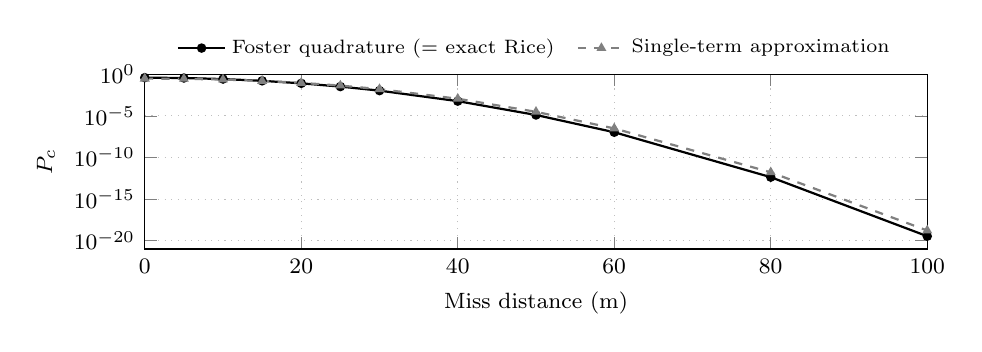
\begin{tikzpicture}
\begin{semilogyaxis}[
  width=0.95\columnwidth, height=3.8cm,
  xlabel={Miss distance (m)}, ylabel={$P_c$},
  xmin=0, xmax=100, ymin=1e-21, ymax=1,
  xtick={0,20,40,60,80,100},
  ytick={1e-20,1e-15,1e-10,1e-5,1},
  grid=major, grid style={dotted,gray!50},
  legend style={at={(0.5,1.03)}, anchor=south, legend columns=2,
                font=\scriptsize, draw=none,
                /tikz/every even column/.append style={column sep=6pt}},
  mark size=1.3pt]
\addplot[black, thick, mark=*] coordinates {
  (0,3.934693e-1)(5,3.572858e-1)(10,2.671202e-1)(15,1.637810e-1)
  (20,8.189230e-2)(25,3.318288e-2)(30,1.082945e-2)(40,5.899491e-4)
  (50,1.279102e-5)(60,1.078641e-7)(80,4.271015e-13)(100,3.413649e-20)};
\addplot[gray, thick, dashed, mark=triangle*, mark options={solid}] coordinates {
  (0,3.032653e-1)(5,2.846208e-1)(10,2.328798e-1)(15,1.621295e-1)
  (20,9.355988e-2)(25,4.383562e-2)(30,1.644326e-2)(40,1.149792e-3)
  (50,3.078554e-5)(60,3.105372e-7)(80,1.642104e-12)(100,1.646977e-19)};
\legend{Foster quadrature (= exact Rice), Single-term approximation}
\end{semilogyaxis}
\end{tikzpicture}
\caption{Collision probability versus miss distance for $\sigma=10$~m per
axis and $\HBR=10$~m. The Foster quadrature coincides with the exact solution
over 19 decades.}
\label{fig:pc}
\end{figure}

\subsection{Physics Validation}

All 18 analytical checks pass in under 0.7~s. Foster agrees with the Rice
solution to $2.3\times10^{-16}$ and with Chan to $4.6\times10^{-16}$ (isotropic)
and $\le1.3\times10^{-3}$ (5:1 and rotated 3.3:1 covariances), relative. Monte
Carlo ($2\times10^{5}$ draws) agrees within four standard errors on all three
geometries, and the Alfano bound ($2.60\times10^{-3}$) exceeds Foster
($2.30\times10^{-3}$), as required. The $J_2$ Runge--Kutta integrator drifts in
energy by $6.7\times10^{-11}$ over 3~h and stays within 0.040~km of SGP4 over
30~min. The Clohessy--Wiltshire, Hohmann, and rocket-equation checks agree with
numerical results to $2.3\times10^{-3}$, $1.6\times10^{-7}$, and
$1.4\times10^{-9}$, and the SBM produces 778 fragments where \eqref{eq:sbm}
predicts 777.6 (800 + 15~kg at 10~km/s).

\subsection{Screening Throughput}

Table~\ref{tab:screen} shows the screening funnel for 500 objects. The KD-tree
search returns 153\,144 candidate pair-steps out of about $1.8\times10^{8}$
(124\,750 pairs at each of 1\,441 epochs). The linear filter keeps 314
pair-steps. After the cap of three refinements per pair, 274 Brent refinements
are run over 240 distinct pairs; 189 of them, covering 165 distinct pairs, end
within 25~km, giving 165 alerts. The funnel is identical across runs, and
end-to-end screening took 0.86--1.00~s over four runs, well inside the 30-s
refresh interval.

Because the bundled TLEs are old at this epoch (median span of the older TLE at
TCA 6.3~days, maximum 25.6~days), the modeled covariance is large and the
maximum $\Pc$ is $7.6\times10^{-8}$. Seven alerts are rated WARNING because
their miss distance is below 5~km, and 158 are rated WATCH. No alert reaches
even the $10^{-7}$ monitor tier, so every decision action is NONE and the
maneuver planner was not triggered in this run; its evaluation rests on the
constructed encounters in Section~\ref{sec:maneuver}. Operational use would
require recent TLEs.

\begin{table}[!t]
\caption{Screening Funnel and Stage Times (500 Objects, 24-h Window)}
\label{tab:screen}
\centering
\footnotesize
\begin{tabular}{@{}lrr@{}}
\toprule
Stage & Output & Time (s) \\
\midrule
SGP4 propagation on 60-s grid & 500 objects & 0.198 \\
KD-tree candidate search & 153\,144 pair-steps & 0.432 \\
Linear relative-motion filter & 314 pair-steps & -- \\
Brent TCA refinement ($\le$3 per pair) & 274 runs & 0.073 \\
Foster $P_c$ and alert assembly & 165 alerts & 0.247 \\
\midrule
Total (representative run) & & 0.950 \\
\bottomrule
\multicolumn{3}{@{}l}{\scriptsize Filter time is included in the Brent row.}
\end{tabular}
\end{table}

\subsection{Maneuver Verification}
\label{sec:maneuver}

Regression tests exercise the planner on constructed encounters. In one test,
the naive minimum-$\Delta v$ burn, executed on a clone of the satellite, brings
the maneuvering satellite within 30~m of a third payload, which full screening
confirms. The planner marks that option as not cascade-safe, matches the
secondary miss distance to within 50~m, and selects a different burn that still
reaches $\Pc<10^{-6}$. In a separate test, the planner's predicted post-burn
miss distance equals the executed result to within 10~m and its predicted TCA
to within 1~s. The two-body Clohessy--Wiltshire along-track drift agrees with
numerical propagation to within 0.5\% (or 2~m) for burns of up to 0.05~m/s over
2~h, and the rocket-equation propellant mass agrees with Runge--Kutta
integration of the mass flow to within $10^{-6}$ relative error.

\subsection{Surrogate Accuracy and Explanations}

Table~\ref{tab:ml} reports held-out results; F1 is the harmonic mean of
precision and recall. The surrogate's mean absolute error (MAE) of 0.106
decades is 15 times lower than that of the miss-distance-only baseline. That
baseline is deliberately weak: it never predicts $\Pc\ge10^{-4}$, which shows
that miss distance alone cannot rank risk when the covariance depends on TLE
age. At the $10^{-6}$ tier the surrogate reaches 0.986 precision and 0.979
recall. Removing the radial miss, or masking features as happens in the live
pipeline, raises the error but keeps F1 above 0.88. Projecting the inputs onto
principal components hurts accuracy, because the features are weakly redundant
(six of seven components are needed for 95\% of the variance) and trees split
along one axis at a time. The mean absolute TreeSHAP contributions show that
the larger TLE age dominates (1.00 decades), because it drives the along-track
covariance. It is followed by miss distance (0.78), HBR (0.57), radial miss
(0.29), and relative speed (0.15), which is consistent with \eqref{eq:cov} and
\eqref{eq:foster}.

\begin{table}[!t]
\caption{Held-Out Surrogate Accuracy (12\,000 Encounters, 1\,931 With
$P_c\ge10^{-4}$)}
\label{tab:ml}
\centering
\footnotesize
\begin{tabular}{@{}lccccc@{}}
\toprule
Model & MAE & RMSE & Prec. & Rec. & F1 \\
\midrule
XGBoost, 7 features      & \textbf{0.106} & \textbf{0.241} & \textbf{0.975} & \textbf{0.950} & \textbf{0.962} \\
\quad without radial miss & 0.224 & 0.634 & 0.971 & 0.924 & 0.947 \\
\quad masked features     & 0.337 & 0.756 & 0.965 & 0.811 & 0.881 \\
\quad first 6 principal comp. & 0.250 & -- & -- & -- & 0.910 \\
Miss-only XGBoost        & 1.565 & 1.879 & 0     & 0     & 0     \\
Constant predictor       & 1.739 & 2.277 & --    & --    & --    \\
\bottomrule
\multicolumn{6}{@{}l}{\scriptsize MAE: mean absolute error; RMSE: root-mean-square
error, both in decades of $P_c$.}\\
\multicolumn{6}{@{}l}{\scriptsize Classification at $P_c\ge10^{-4}$. --: not computed.}
\end{tabular}
\end{table}

\subsection{Negative Results}

Two learned components were evaluated and excluded from the decision path. A
12-unit ungated Elman recurrent network~\cite{elman1990} for trajectory
prediction reaches a position MAE of 459~km on 512 test sequences. That is worse than both
persistence (347~km) and linear extrapolation (20.5~km), so it is labeled
experimental and feeds no alert. Two graph rankers, a summary-statistics
network and a four-head graph attention network~\cite{velickovic2018},
reach 98.8\% and 95.5\% accuracy on synthetic
graphs, but their labels come from a heuristic, which makes those scores
circular. On the 500-object benchmark graph, the attention ranker's Spearman
correlation with the physics $P_{\mathrm{hit}}$ is only 0.14, and the two
rankers disagree with each other by up to 0.38 in probability. They are
therefore shown only as an advisory cross-check and never set depth,
probability, or the maneuver plan.

%% ==========================================================================
\section{Discussion and Limitations}
\label{sec:discussion}

The design keeps the physical $\Pc$ separate from learned estimates, and the
negative results show why baselines matter: without them, the recurrent network
and the two graph models would have appeared useful. The system has important
limitations. The covariance is modeled from TLE age
rather than taken from CDMs, so absolute $\Pc$ values are only as good as
\eqref{eq:cov}~\cite{alfriend1999,hall2019}. Object masses are assumed, because
SATCAT provides none, and they set the SBM fragment count through $M^{0.75}$.
The surrogate is trained on synthetic geometry with combined radii of 3--50~m,
whereas live combined radii are often below 3~m. On the 500-object benchmark
its median disagreement with the physics $\Pc$ is 0.90 decades, mostly for
$\Pc<10^{-7}$, where training labels are floored; its held-out accuracy
therefore measures how well it reproduces the physics on the training
distribution, not operational skill. The planner checks each alert's options
independently, so two simultaneous burns are not screened against each other,
and burns are impulsive. Throughput was measured for 500 objects; candidate
counts grow roughly quadratically with catalog size, so a full catalog would
require parallelization. Future work includes validation on real CDM
sequences~\cite{uriot2022}, comparison with the CARA tools~\cite{caratools},
and multi-burn coordination.

%% ==========================================================================
\section{Conclusion}
\label{sec:conclusion}

Orbital Sentinel couples future-window screening, cross-checked Foster
collision probability, NASA SBM fragment screening, an alert-based cascade
graph, and maneuver planning that rejects burns that create new conjunctions in
one open pipeline. Its probability engine matches the exact solution over 19
decades, it screens 500 objects in about one second on a laptop processor, and
it passes 18 analytical checks and 204 regression tests. The explainable
surrogate reaches 0.106-decade error with 0.95 recall at the maneuver threshold
but can never lower the physics action. The source code is available at
\url{https://github.com/Pritam-mb/orbit-sentinal}.

%% ==========================================================================
\section*{Author Contributions (CRediT)}
\textbf{Soumyadeep Dey:} Conceptualization, Methodology, Software, Validation,
Formal analysis, Writing -- original draft.
\textbf{Pritam Patra:} Software, Visualization, Project administration,
Writing -- original draft, Writing -- review \& editing.
\textbf{Subarna Maity:} Software, Visualization.
\textbf{Sourish Panda:} Investigation, Writing -- review \& editing.

\section*{Acknowledgment}
The authors thank CelesTrak and the U.S. Space Force Space-Track service for
publicly available TLE and SATCAT data, and the maintainers of the open-source
sgp4, SciPy, XGBoost, PyTorch, and CesiumJS projects.

%% ==========================================================================
\begin{thebibliography}{99}

\bibitem{esa2026}
ESA Space Debris Office, ``ESA's annual space environment report,'' ESA ESOC,
Darmstadt, Germany, Rep. GEN-DB-LOG-00288-OPS-SD, Iss. 10.1, Sept. 2026.
[Online]. Available:
\url{https://www.sdo.esoc.esa.int/environment_report/Space_Environment_Report_I10R1_20260908.pdf}

\bibitem{esastats2026}
ESA Space Debris Office, ``Space environment statistics,'' DISCOSweb, ESA
ESOC. Accessed: Oct. 12, 2026. [Online]. Available:
\url{https://sdup.esoc.esa.int/discosweb/statistics/}

\bibitem{kelso2009}
T. S. Kelso, ``Analysis of the Iridium 33--Cosmos 2251 collision,'' in
\emph{Proc. AAS/AIAA Astrodyn. Specialist Conf.}, Pittsburgh, PA, USA,
Aug. 2009, Paper AAS 09-368.

\bibitem{kessler1978}
D. J. Kessler and B. G. Cour-Palais, ``Collision frequency of artificial
satellites: The creation of a debris belt,'' \emph{J. Geophys. Res.},
vol.~83, no.~A6, pp.~2637--2646, June 1978, doi: 10.1029/JA083iA06p02637.

\bibitem{liou2006}
J.-C. Liou and N. L. Johnson, ``Risks in space from orbiting debris,''
\emph{Science}, vol.~311, no.~5759, pp.~340--341, Jan. 2006,
doi: 10.1126/science.1121337.

\bibitem{nasa2020}
NASA, ``NASA spacecraft conjunction assessment and collision avoidance best
practices handbook,'' NASA, Washington, DC, USA, NASA/SP-20205011318,
Dec. 2020. [Online]. Available:
\url{https://ntrs.nasa.gov/citations/20205011318}

\bibitem{uriot2022}
T. Uriot \emph{et al.}, ``Spacecraft collision avoidance challenge: Design and
results of a machine learning competition,'' \emph{Astrodynamics}, vol.~6,
no.~2, pp.~121--140, June 2022, doi: 10.1007/s42064-021-0101-5.

\bibitem{sanchez2021}
L. S\'{a}nchez Fern\'{a}ndez-Mellado and M. Vasile, ``On the use of machine
learning and evidence theory to improve collision risk management,''
\emph{Acta Astronaut.}, vol.~181, pp.~694--706, Apr. 2021,
doi: 10.1016/j.actaastro.2020.08.004.

\bibitem{stevenson2023}
E. Stevenson, V. Rodriguez-Fernandez, H. Urrutxua, and D. Camacho,
``Benchmarking deep learning approaches for all-vs-all conjunction
screening,'' \emph{Adv. Space Res.}, vol.~72, no.~7, pp.~2660--2675,
Oct. 2023, doi: 10.1016/j.asr.2023.01.036.

\bibitem{hoots1980}
F. R. Hoots and R. L. Roehrich, ``Models for propagation of NORAD element
sets,'' Aerospace Defense Command, U.S. Air Force, Peterson AFB, CO, USA,
Spacetrack Rep. No.~3, Dec. 1980. [Online]. Available:
\url{https://celestrak.org/NORAD/documentation/spacetrk.pdf}

\bibitem{vallado2006}
D. A. Vallado, P. Crawford, R. Hujsak, and T. S. Kelso, ``Revisiting
Spacetrack Report \#3,'' in \emph{Proc. AIAA/AAS Astrodyn. Specialist Conf.
Exhib.}, Keystone, CO, USA, Aug. 2006, Paper AIAA 2006-6753,
doi: 10.2514/6.2006-6753.

\bibitem{flohrer2008}
T. Flohrer, H. Krag, and H. Klinkrad, ``Assessment and categorization of TLE
orbit errors for the US SSN catalogue,'' in \emph{Proc. Adv. Maui Opt. Space
Surveill. Technol. Conf. (AMOS)}, Maui, HI, USA, Sept. 2008, pp.~513--524.

\bibitem{vallado2012}
D. A. Vallado and P. J. Cefola, ``Two-line element sets---Practice and use,''
in \emph{Proc. 63rd Int. Astronaut. Congr. (IAC)}, Naples, Italy, Oct. 2012,
pp.~5812--5825.

\bibitem{hoots1984}
F. R. Hoots, L. L. Crawford, and R. L. Roehrich, ``An analytic method to
determine future close approaches between satellites,'' \emph{Celest.
Mech.}, vol.~33, no.~2, pp.~143--158, 1984.

\bibitem{foster1992}
J. L. Foster and H. S. Estes, ``A parametric analysis of orbital debris
collision probability and maneuver rate for space vehicles,'' NASA Johnson
Space Center, Houston, TX, USA, Tech. Rep. JSC-25898, Aug. 1992.

\bibitem{chan2008}
F. K. Chan, \emph{Spacecraft Collision Probability}. El Segundo, CA, USA:
Aerospace Press, 2008, doi: 10.2514/4.989186.

\bibitem{patera2001}
R. P. Patera, ``General method for calculating satellite collision
probability,'' \emph{J. Guid. Control Dyn.}, vol.~24, no.~4, pp.~716--722,
July 2001, doi: 10.2514/2.4771.

\bibitem{akella2000}
M. R. Akella and K. T. Alfriend, ``Probability of collision between space
objects,'' \emph{J. Guid. Control Dyn.}, vol.~23, no.~5, pp.~769--772,
Sept. 2000, doi: 10.2514/2.4611.

\bibitem{alfriend1999}
K. T. Alfriend, M. R. Akella, J. Frisbee, J. L. Foster, D.-J. Lee, and
M. Wilkins, ``Probability of collision error analysis,'' \emph{Space Debris},
vol.~1, no.~1, pp.~21--35, Mar. 1999, doi: 10.1023/A:1010056509803.

\bibitem{hall2019}
D. T. Hall, ``Implementation recommendations and usage boundaries for the
two-dimensional probability of collision calculation,'' in \emph{Proc.
AAS/AIAA Astrodyn. Specialist Conf.}, Portland, ME, USA, Aug. 2019,
Paper AAS 19-632.

\bibitem{hall2018}
D. T. Hall, S. J. Casali, L. C. Johnson, B. B. Skrehart, and L. G. Baars,
``High fidelity collision probabilities estimated using brute force Monte
Carlo simulations,'' in \emph{Proc. AAS/AIAA Astrodyn. Specialist Conf.},
Snowbird, UT, USA, Aug. 2018, Paper AAS 18-244.

\bibitem{caratools}
NASA CARA, ``CARA Analysis Tools,'' GitHub repository. Accessed: Oct. 12,
2026. [Online]. Available: \url{https://github.com/nasa/CARA_Analysis_Tools}

\bibitem{kelso2006}
T. S. Kelso and S. Alfano, ``Satellite orbital conjunction reports assessing
threatening encounters in space (SOCRATES),'' in \emph{Proc. SPIE, Modeling,
Simulation, and Verification of Space-Based Systems III}, vol.~6221,
May 2006.

\bibitem{peng2020}
H. Peng and X. Bai, ``Machine learning approach to improve satellite orbit
prediction accuracy using publicly available data,'' \emph{J. Astronaut.
Sci.}, vol.~67, no.~2, pp.~762--793, June 2020,
doi: 10.1007/s40295-019-00158-3.

\bibitem{lundberg2020}
S. M. Lundberg \emph{et al.}, ``From local explanations to global
understanding with explainable AI for trees,'' \emph{Nat. Mach. Intell.},
vol.~2, no.~1, pp.~56--67, Jan. 2020, doi: 10.1038/s42256-019-0138-9.

\bibitem{chen2016}
T. Chen and C. Guestrin, ``XGBoost: A scalable tree boosting system,'' in
\emph{Proc. 22nd ACM SIGKDD Int. Conf. Knowl. Discov. Data Mining}, San
Francisco, CA, USA, Aug. 2016, pp.~785--794, doi: 10.1145/2939672.2939785.

\bibitem{johnson2001}
N. L. Johnson, P. H. Krisko, J.-C. Liou, and P. D. Anz-Meador, ``NASA's new
breakup model of EVOLVE 4.0,'' \emph{Adv. Space Res.}, vol.~28, no.~9,
pp.~1377--1384, 2001, doi: 10.1016/S0273-1177(01)00423-9.

\bibitem{velickovic2018}
P. Veli\v{c}kovi\'{c}, G. Cucurull, A. Casanova, A. Romero, P. Li\`{o}, and
Y. Bengio, ``Graph attention networks,'' in \emph{Proc. Int. Conf. Learn.
Represent. (ICLR)}, 2018. [Online]. Available:
\url{https://arxiv.org/abs/1710.10903}

\bibitem{bentley1975}
J. L. Bentley, ``Multidimensional binary search trees used for associative
searching,'' \emph{Commun. ACM}, vol.~18, no.~9, pp.~509--517, Sept. 1975,
doi: 10.1145/361002.361007.

\bibitem{brent1973}
R. P. Brent, \emph{Algorithms for Minimization Without Derivatives}.
Englewood Cliffs, NJ, USA: Prentice-Hall, 1973.

\bibitem{virtanen2020}
P. Virtanen \emph{et al.}, ``SciPy 1.0: Fundamental algorithms for scientific
computing in Python,'' \emph{Nat. Methods}, vol.~17, no.~3, pp.~261--272,
Mar. 2020, doi: 10.1038/s41592-019-0686-2.

\bibitem{alfano2005b}
S. Alfano, ``Relating position uncertainty to maximum conjunction
probability,'' \emph{J. Astronaut. Sci.}, vol.~53, no.~2, pp.~193--205, 2005.

\bibitem{clohessy1960}
W. H. Clohessy and R. S. Wiltshire, ``Terminal guidance system for satellite
rendezvous,'' \emph{J. Aerosp. Sci.}, vol.~27, no.~9, pp.~653--658,
Sept. 1960, doi: 10.2514/8.8704.

\bibitem{elman1990}
J. L. Elman, ``Finding structure in time,'' \emph{Cogn. Sci.}, vol.~14,
no.~2, pp.~179--211, Mar. 1990, doi: 10.1207/s15516709cog1402\_1.

\end{thebibliography}

\end{document}
